%!TEX root = ../Thesis.tex
\chapter{Predict permeation enhancement}

A main goal of this thesis has been to use the preclinical data more efficiently. Instead of testing randomly new absorption enhancers or what intuitively seems promising, a model built on previous experiences, can fast systematically evaluate larger libraries of molecules.

\subsection{Work flow and early challenges}
\label{predPerm:workflow}

Very early in the project three areas to predicts were identified. These were solubility, critical micelle concentration (CMC) and permeation enhancement. In Novo Nordisk for purposes securing intellectual properties, the default rule is that no in-house data generated by the drug development projects can be published. Therefore all data used in this PhD thesis was already public available from third-party sources or conducted in experiments for this thesis only. 

Figure \ref{predict_workflow} outline the the work flow in to build models to predict permeation enhancement.

\begin{figure}[!htbp]
\label{predict_workflow}
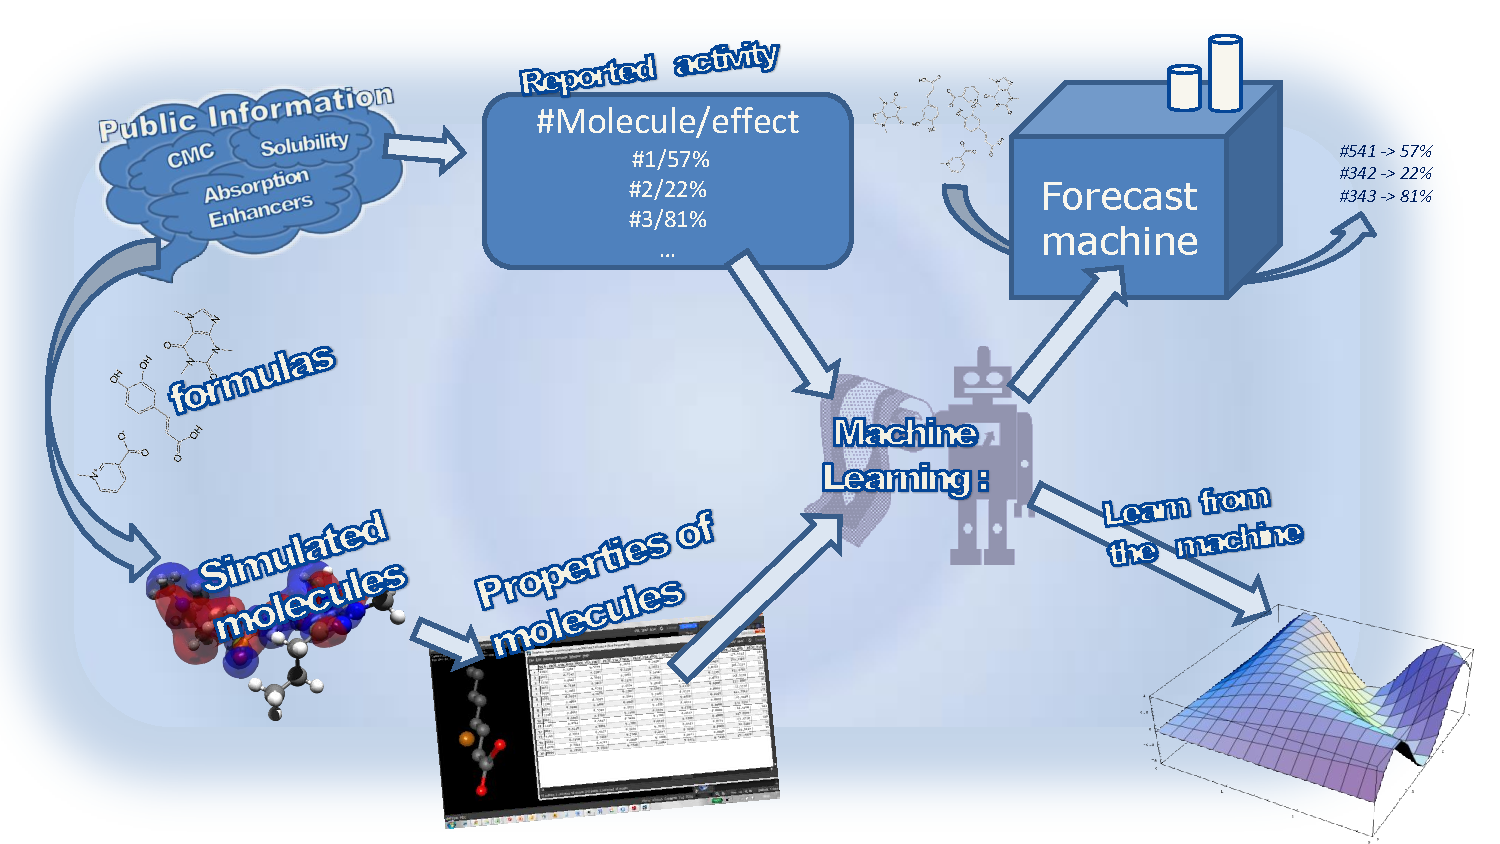
\includegraphics[width=\textwidth, height=\textheight, keepaspectratio]{graphics/predictPotencySummary.pdf}
\caption{Outline how to predictions are made. This figure was first designed for PhD-related presentations given by the author.}
\end{figure}

The work flow outline a bottom up approach where very simple \textit{in-vitro} experiments are conducted for series of candidates molecules. Each molecular formula is at the same time characterized by computed molecular descriptors  produced training features. With machine learning a relationship is established between the molecular formula and the \textit{in-vitro} response.

Data on \textit{in-vitro} Caco-2 permeation enhancement or similar pre-clinical studies were not expected alone to be useful to select new enhancers. As discussed in Section \ref{someWhere} \text{in-vitro} studies tend to overestimate the importance and impact of lipophilicity in absorption enhancers. Enhancers with C16 carbon chains are found 10-50 fold more potent than their C10 counter parts. Nevertheless C16 carbon chain based permeation enhancer, have quite disappointing not delivered the same potency in \textit{in-vivo} studies. An obvious testimony is that there is no public announced clincal trials using C16 surfactant peptide absorption enhancers \cite{aguirre2016current}.

It was noted that in CMC was correlated with high absorption potency(citations needed). Initially to collect data sets on CMC values was a central part. However,  I found no litterature that in fact shows, that low CMC values directly should cause permeation enhancement. Rather CMC is simply being one of more collective attributes associated with lipophilicity \cite{rosen2012surfactants} and surfactant can be effective below their CMC \cite{xia2000mechanistic}. Therefore, it would make more sense to build predictive models using a target that resembled the permeation enhancement the most. Therefore Caco-2 measurements was finally favored over CMC determination.

Molecular solubility in watery buffers is not surprisingly negatively associated with lipophilicity / hydrophibicity. In a worst case scenario potency predictions and solubility predictions would be highly negatively correlated. Then to the model permeation potency and in-solubility would be indistinquisble phenomena. In such case the the combined solubility and permeation enhancement model, would be to identify both soluble and relatively potent permeation enhancers. \textit{vice versa}.

\subsection{Challenges of a top down modeling of permeation enhancement}
In opposite to the bottom approach modeling simplified \textit{in-vitro} experiments a top down approach was also being fallowed in the project. Instead,
a devised hypothesis was, that molecules claimed in literature such as articles and patent applications to permeation enhancers could be used as training examples, of how an permeation enhancer should look like.

One data set was obtained in an effort to use text mining to collect examples of compounds being mentioned for being permeation enhancers and/or absorption enhancers. The data set was aquirred as a part of Sarah Brebbia Dirksen (Øster) master thesis project in 2012. A list of 167 compounds originating from patent applications and research articles was compiled. \cite{sara2012application}.

Such a set of examples would not only reflect \textit{in-vitro} studies, but also a series of unknown limitations such as toxicology, formulation in-capabilities etc. Thus a model build on target data in the end stage of process, may contain a number of favorable biases, such that the model tend not to suggest toxic molecules as permeations enhancers.

It was assumed that permeation enhancement is a rare property of molecules, such that any random molecule would likely not be an enhancer. Random molecules of similar weight was acquired from a (compound DATABASE). With the software packages ACDlabs and Molecular operating environment, 49 chemical descriptors was computed for both sets of molecules and linear discriminant analysis has been used to learn a class separation rule to identify typical enhancer like molecules. \cite{sara2012application}

Although a valid cross-validation of the classification model predicted a nearly perfect classification accuracy, sensitivity and recovery, the model failed in a proof of concept to test predicted molecules in-house in the Caco-2 model. There are a number reasons why this approach can have failed in spite of a promising cross-validation. To be fair some of these reasons were mentioned in the fine master thesis, however in the clear light of hind sight, let us in the following run through the assumptions of supervised machine learning cross-validation.

\subsection{Identical distributions}
A requirement was that training and future test observations had to be drawn from same distributions. The training set originated with positive examples from the pharmaceutical litterature and with negative examples from what appear to be a random synthesis chemical library. It was assumed that all molecules from random synthesis library were not effective as enhancers, and I agree on this as a plausible assumption. However visually inspecting the random synthesis molecules, reveal these molecules were far from typical excipients in pharmaceutical. Exotic heavy atoms as uranium! or what appear to be a truly random pattern of substitutions. If this library infact was generated as an random or an exhaustive search of possible molecule graphs below a given molar weight, then average molecule will look far from the typical excipients in pharmaceutical industry. The typical excipient, especially surfactant enhancers, are not very substituted, not very branched. If generating a molecule starting from one carbon atom, and any choice has equal probability, should this carbon chain branch out here or not? should there be substituted something here or not? the molecules end being very branched and highly substituted, simply because the simply relatively few combinations of molecules that have long non branched non substituted carbon chains. Thus the classification model have been trained to recognize the difference between two groups of molecule that are obviously different. A part of the reason the two classes of molecules are different in the training may well being an permeation enhancer or not. However any other differences will be confounded. Most likely such classification model would be used to scan through a library of approved pharmaceutical excipients, thus only drawing observations to predict from the pharmaceutical molecule distribution. Suddenly the model may recognize many of the molecules as permeation enhancers, simply because these are not branched enough or highly substituted.

\subsection{Anticipated complexity enhancement mechanisms robust estimation.}


\section{}




\begin{figure}[htbp]
\label{workSummary}
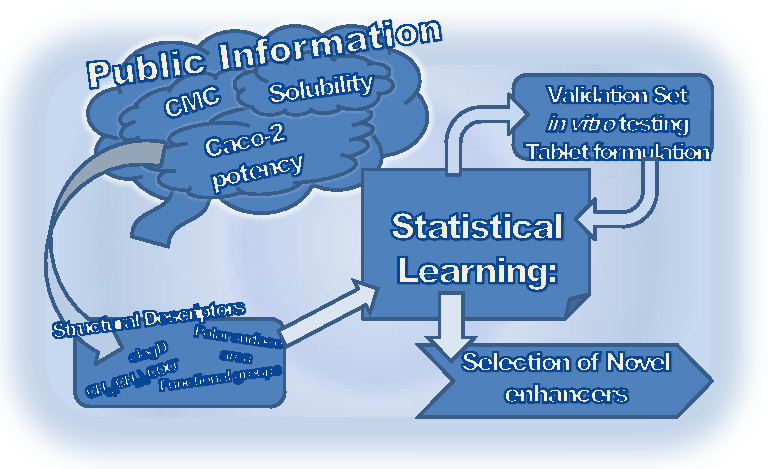
\includegraphics{graphics/workSummary_130mm.pdf}
\caption{Project idea. This figure was first designed for PhD-related presentations given by the author.}
\end{figure}

\begin{figure}[ht]
\label{devel_fassif}
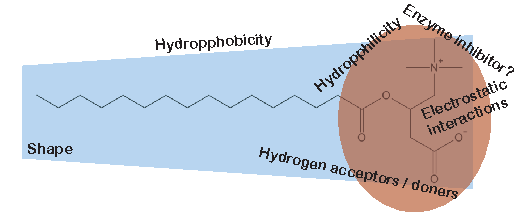
\includegraphics{graphics/typeOfSurfactant.pdf}
\caption{how does a surfactant like enhancer look like. This figure was first designed for PhD-related presentations given by the author.}
\end{figure}

\begin{figure}[ht]
\label{devel_fassif}
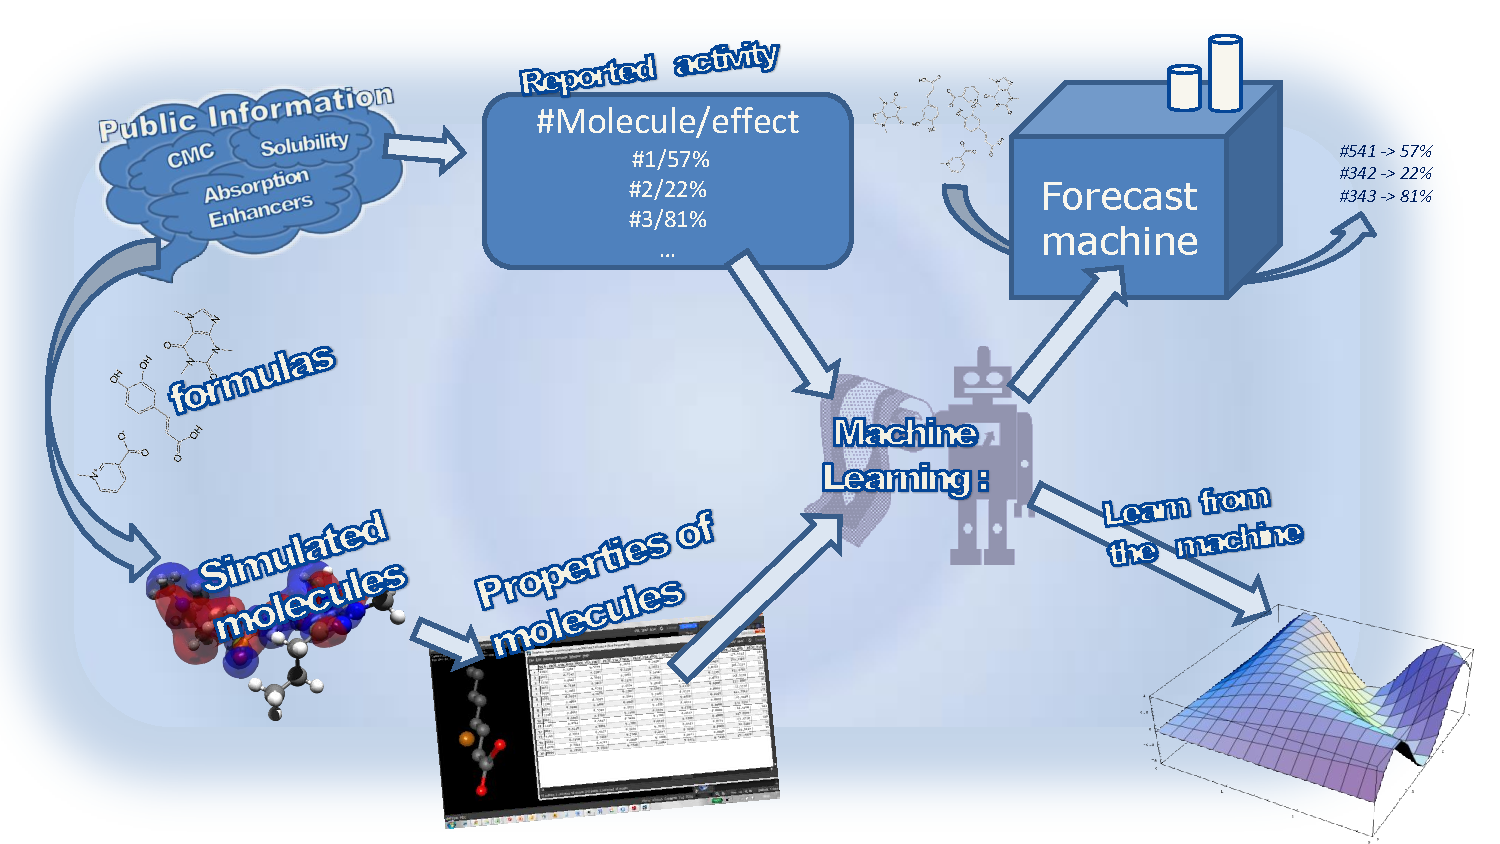
\includegraphics[width=\textwidth, height=\textheight, keepaspectratio]{graphics/predictPotencySummary.pdf}
\caption{Outline how to predictions are made. This figure was first designed for PhD-related presentations given by the author.}
\end{figure}

The decision tree ensemble random forest have a series of useful diagnostics which have been used in this thesis work.

\section{Article: In silico modelling of permeation enhancement potency in Caco-2
monolayers based on molecular descriptors and random forest}

\newpage

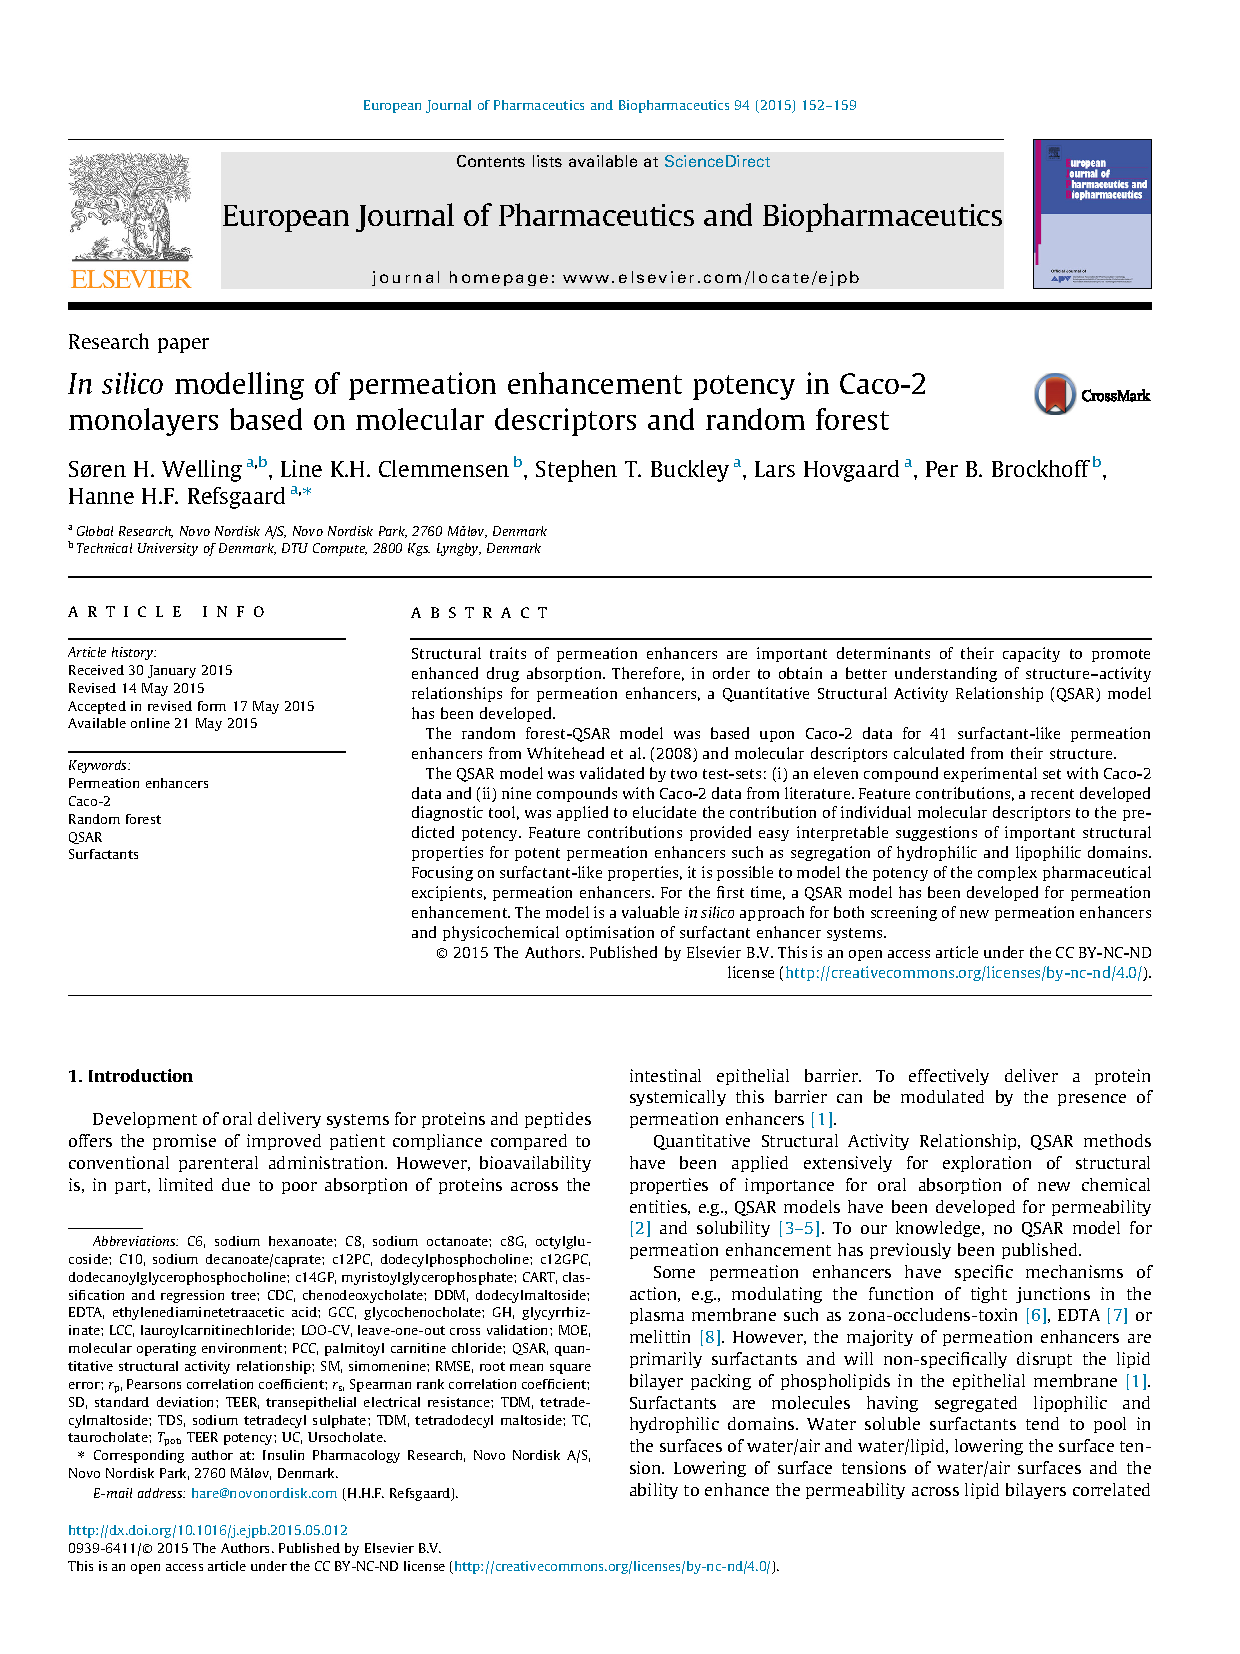
\includepdf[pages={1-},scale=0.90,pagecommand={\pagestyle{myruled}}]{chapters/predictPotencyArt.pdf}


